\section{Remarks on Tomberg}

\begin{wrapfigure}{rt}{.3\textwidth}
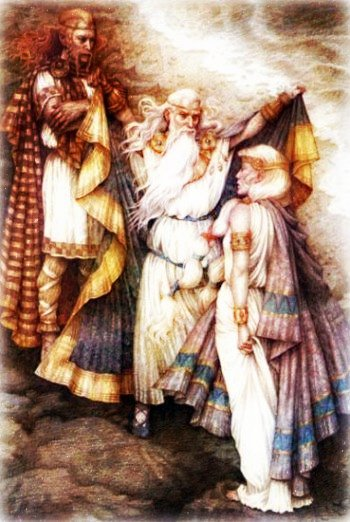
\includegraphics[width=.3\textwidth]{Conn252Cdruidaymujer.jpg}
\end{wrapfigure}

Those who are interested in reading Meditations ought to peruse this index to his book here\footnote{\url{http://www.beautytruegood.co.uk/tarotdex.htm\#G}}. Consulting the index under ``personal magic'', one is referred to pages 478-480 (among others):

\begin{quotex}
Therefore, it follows from the preceding that magical formulae are not invented -- just as true poetry is not invented -- but that they are born from blood and light. This is why one uses in sacred magic, as a rule, traditional formulae -- and this not because they are ancient, but rather because they took birth in the above indicated manner and they have proved themselves as such. This was well known to Martines de Pasqually, for example. The rituals of his magical invocations consist only of traditional formulae, drawn above all from the Psalms -- not because he was a practicing Catholic but solely in view of heir magical effectiveness (int eh magic that he taught and practiced). Sacred magic differs from personal or arbitrary magic -- beyond the differences which we have stated in the third Letter -- also in that it ``makes use'' of the agent of growth, whilst arbitrary magic works above all with the magical agent of electricity... neither science nor personal magic can perform miracles... on the other hand, every human word can become magical if it is sincere to the point of engaging the blood, and if at the same point it is filled by faith to the point of setting the luminous waters of hope from above in motion.
\end{quotex}


Tomberg is not rejecting paganism or magic per se (such as that outlined by the UR Group in their essays with Evola on magic, or by Franz Bardon in his work); he is endeavoring to place it within the Empire of Heaven. Just as traditionalism finds its fulfillment in the notion of an Imperium or sacral Emperorship which guarantees the ``shields of the earth'' (kingdoms) by stepping even higher, so does Tomberg push Eastern mysticism into the ``Selves beyond the Selves'' \& the ``Magic from on high'' which supersedes without annihilating all lesser shadows and analogies.

Tomberg quotes Christ in the Beatitudes, who says:

\begin{quotex}
Matthew 5:33 Again, ye have heard that it hath been said by them of old time, Thou shalt not forswear thyself NKJV: swear falsely , but shalt perform unto the Lord thine oaths: 34 But I say unto you, Swear not at all; neither by heaven; for it is God's throne: 35 Nor by the earth; for it is his footstool: neither by Jerusalem; for it is the city of the great King. 36 Neither shalt thou swear by thy head, because thou canst not make one hair white or black. 37 But let your communication be, Yea, yea; Nay, nay: for whatsoever is more than these cometh of evil.
\end{quotex}

Rather than being a prohibition of any oaths, or magic, Tomberg interprets this as being a temporary injunction which is absolute until the proper ``centers'' (inner/outer) are restored. It is a question of our lack of knowledge -- the only kind of personal magic that un-illumined man can ``reach'' is serpentine and purely horizontal -- thus, it represents only a deepening of his plight. However, once the relationship with the ``waters above the earth'' is restored, it is a different question. God prohibits because we are not ready.

There is a significant link here with the following idea from Hebrews 6:

\begin{quotex}
For when God made the promise to Abraham, since He could swear by no one greater, He swore by Himself, saying, ``I WILL SURELY BLESS YOU AND I WILLSURELY MULTIPLY YOU. And so, having patiently waited, he obtained the promise. For men swear by one greater than themselves, and with them an oath given as confirmation is an end of every dispute. In the same way God, desiring even more to show to the heirs of the promise the unchangeableness of His purpose, interposed with an oath, so that by two unchangeable things in which it is impossible for God to lie, we who have taken refuge would have strong encouragement to take hold of the hope set before us. This hope we have as an anchor of the soul, a hope both sure and steadfast and one which enters within the veil, where Jesus has entered as a forerunner for us, having become a high priest forever according to the order of Melchizedek.
\end{quotex}


The double oath is found on the tablet of Enoch, who walked with God-

\emph{As above, so below.}


Man's destiny is to have what he wants, but in God's way, and God's time. This is the mystery of the ``Self beyond the Self'', which only the ``Self'' can find.


\flrightit{Posted on 2012-01-28 by Logres}

